
\chapter{Clustering}
\label{Clustering}

Clustering algorithms divide a dataset into several disjoint subsets. All elements in such
a subset share common features like, for example, spatial proximity.
Clustering is used as a stand-alone tool to get insight into the distribution
of a data set or as a preprocessing step for other algorithms operating on the
detected clusters. The former can be used to determine stop
criteria (see section 3.2) and the latter is used in our deterioration
schema (see chapter 4).

\section{Cluster Extension}

Basin of attraction is a term used in dynamic systems
defined as the set of initial conditions leading to long-time 
behavior that approaches the particular attractor.
In the field of global optimization, basin of attraction may
be defined in the following way.

\begin{definition}\label{def:basin}
\textbf{Basin of attraction} is a subset A of the problem space which contains
local solution and for each point which belongs to A the gradient of the objective
function at that point will lead towards the solution.
\end{definition}

Clusters may be seen as an approximation of the basin of attraction, because
the distribution of individuals which flooded to the basins
provides useful information about its size and shape. So the clustering 
algorithm may be used to detect the set of individuals which belongs
to the same basin of attraction. Such a set may be later described by extracting
some statistical information from that set, e.g the center point,  
the radius of the set, covariance matrix etc. This is what we called
a \textbf{Cluster extension}. 
Not only does our algorithm efficiently solve multimodal problems, it also
provides information about detected sets (basins of attraction) in the from 
of cluster extensions. 

\section{Clustering as a Stop Criterion}

The termination criterion in classic evolutionary algorithms is hard to define
and very often problem dependent, as we do not have any global information about 
the fitness landscape and therefore we can only compare one solution to another
previously found. 
Some of the common termination criteria such as: 
\begin{itemize}
  \item maximum computation time
  \item total number of iterations
  \item no improvement for a specified number of iterations
\end{itemize}
are only applicable to a specific problems and none of them can be used
as a general stop criterion. 
The clustering, which is performed in every iteration, 
on the other hand may give us some clues about the global
characteristics of the fitness landscape i.e. when the clustering algorithm performed 
on the final population finds nothing it is very likely that in previous
iterations we have deteriorated the fitness landscape in places where 
the most desirable solutions reside and there is no use in continuing the
searching process. This is considered to be true because we are looking for
robust solutions which are resistant to noise and lie in basins of attraction 
which are significantly wide and deep. The population of EA is likely 
to converge to such solutions, so having found no clusters of individuals after
performing the EA in a given iteration shows that the population does not converge 
to any robust solution. In such circumstances we terminate the main loop
of the algorithm.

\section{OPTICS}

We have choosen density-base clustering algorihtm called \textit{OPTICS:
Ordering Points To Identify the Clustering Structure} \cite{optics}. In density
clustering clusters are regarded as regions in the data space in which the objects are 
dense and which are separated by regions of low object density. These regions
may have an arbitrary shape and the points inside a region may be arbitrarily
distributed.

\textit{OPTICS} is an extendsion to a well-known density clustering algorithm
called \textit{DBSCAN}. The basic idea for \textit{DBSCAN} is that for each
point of a cluster the neighborhood of a given radius $\epsilon$ has to contain
at least a minimum number of points $minPts$.

\textit{OPTICS} works like \textit{DBSCAN} but for an infinite number of
distance paramters $\epsilon_i$ which are smaller than a \textit{generating distance}
$\epsilon$. The only difference is that we do not assing cluster memberships.
Instead, we store the \textbf{order} in which the objects are processed (the
main priniple is that we always have to select an object which is
density-reachable with respect to the lowest $\epsilon$ value to guarantee that
clusters with higher density are finished first) and the information which would
be used by \textit{DBSCAN} algorithm to assing cluster memberships. This
information consists of only two values for each object: \textit{core-distance}
and \textit{reachability-distance}.


\begin{definition}\label{def:core-distance} 
\textbf{core-distance} - the core-distance of an object $p$
is simply the smallest distance $\epsilon'$ between $p$ and an object in its
$\epsilon$-neighborhood such that $p$ would be a core object with respect to
$\epsilon'$ if this neighbor is contained in $N_\epsilon(p)$. Otherwise, the
core-distance is \textit{UNDEFINED}
\end{definition}


\begin{definition}\label{def:reachability-distance} 
\textbf{reachability-distance} - the reachability-distance
of an object $p$ with respect to another object $o$ is the smallest distance such that $p$ is
directly density-reachable from $o$ if $o$ is a core object
\end{definition}

This information is sufficient to extract all density-based clusterings
with respect to any distance $\epsilon'$ which is smaller that the generating
distance $\epsilon$

An advantage of cluster-ordering a data set compared to other clustering methods
is that the ordering which might be visualized by \textit{reachability-plot} of
ordered points is rather insensitive to the input parameters of the method i.e.
the \textit{generating distance} $\epsilon$ and the value for $minPts$. Roughly
speaking, the values have just to be \textit{large} enough to yield a good
result. The concrete values are not crucial because there is a broad range of
possible values for which we always can see the clustering structure of a data
set when looking at the corresponding \textit{reachability-plot}. Figure 3.1
shows the result of \textit{OPTICS} clustering for a sample set of points.
Figure 3.2 shows reachablity plot for various \textit{generating distances} -
$\epsilon$. 

The next chapter describes how \textit{OPTICS ordering} properties are used
to prevent degradation of areas which have not been explored during the course
of the algorithm. 

\begin{figure}
  \centering
  \fbox{
    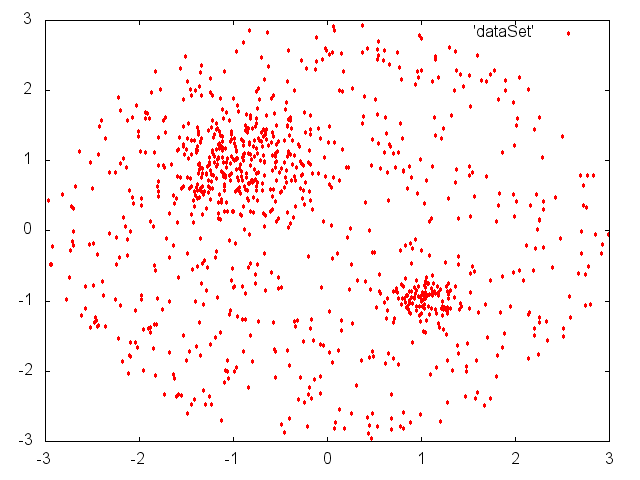
\includegraphics[scale=0.4]{dataSet.png}
  }
  \fbox{
    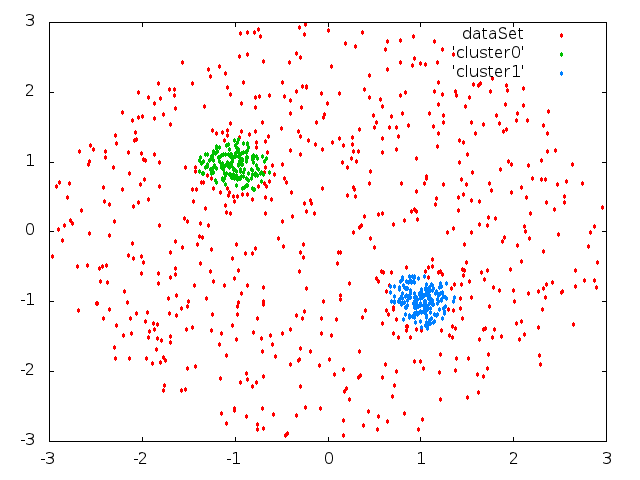
\includegraphics[scale=0.4]{clusters.png}
  }
  \caption{Visualization of the DBSCAN algorithm applied to Optics ordering
  of simple 2-dimensional data set which consists of 1000 points. Optics
  paramters: $minPts=20, \epsilon=1.2$, the two clusters was found using DBSCAN
  paramters: $\epsilon'=0.2$ }
  \label{clusters}
\end{figure}


\begin{figure}
  \centering
  \fbox{
    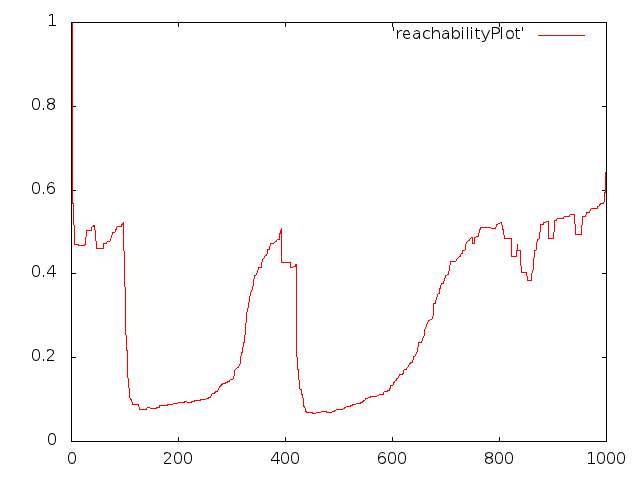
\includegraphics[scale=0.4]{reachability1/1_5_20.png}
  }
  \fbox{
    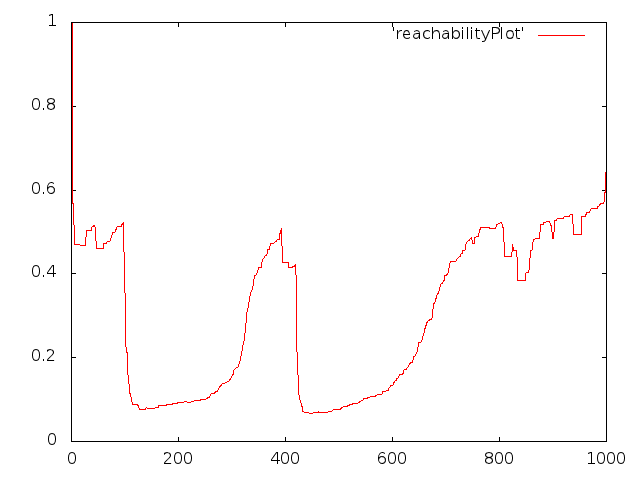
\includegraphics[scale=0.4]{reachability1/1_0_20.png}
  }
  \fbox{
    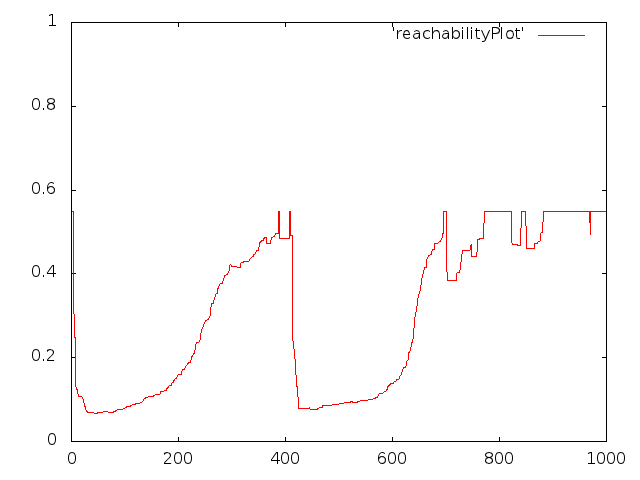
\includegraphics[scale=0.4]{reachability1/0_5_20.png}
  }
  \caption{Reachability plot for data set presented on figure 3.1. Optics
  paramters (minPts, $\epsilon$) are: (20, 1.5), (20, 1.0), (20, 0.5)
  respectively. The two cavities which are visible in each plot depict the two
  of the clusters on figure 3.1. This proves that there is a large range of
  values for $\epsilon$ (\textit{generating distance}) for which the appearance
  of the reachability plot will not change significantly. (the flat shape of function from the last plot
  results from the fact that we truncate the reachability-distance to the 
  generating distance $\epsilon$, when the former is greater than the latter)}
  \label{reach}
\end{figure}